\documentclass[10pt]{article}
\usepackage{arxiv}
\usepackage[round,authoryear]{natbib}
\usepackage{amsmath,amssymb,booktabs,array}
\usepackage{tikz}
\usetikzlibrary{arrows.meta,positioning,fit,backgrounds}
\usepackage{enumitem}
\usepackage{placeins}
\usepackage{xcolor}
\usepackage[colorlinks=true,allcolors=blue!45!black,breaklinks=true]{hyperref}
\usepackage{url}
\urlstyle{same}
% Generated by scripts/numbers.py; do not edit.
\newcommand{\RegressionTarget}{15}
\newcommand{\SituationCount}{5}
\newcommand{\HeldoutTarget}{20}
\newcommand{\SynthTarget}{100,000}
\newcommand{\ChallengeMinimum}{150}
\newcommand{\FirstCardTarget}{1.500}
\newcommand{\ColdTarget}{5}
\newcommand{\CachedTarget}{1}
\newcommand{\ChallengeLimit}{10}
\newcommand{\RetrievalSmallK}{5}
\newcommand{\RetrievalLargeK}{10}
\newcommand{\SequenceLimit}{512}
\newcommand{\TrainingMinuteCap}{45}
\newcommand{\RegressionPassed}{12}
\newcommand{\RegressionTotal}{15}
\newcommand{\SuitePassed}{3}
\newcommand{\ColdMaxSeconds}{12.323}
\newcommand{\WarmMaxSeconds}{12.007}
\newcommand{\CachedMaxSeconds}{0.092}
\newcommand{\TimingCount}{5}
\newcommand{\CacheHits}{1}
\newcommand{\TraceChecked}{296}
\newcommand{\TraceViolations}{0}
\newcommand{\ComposedChecked}{0}
\newcommand{\ComposedFailures}{0}
\newcommand{\ContradictionsFound}{5}
\newcommand{\ClarificationsFound}{3}
\newcommand{\FalseAlarms}{0}
\newcommand{\DocumentCount}{8}
\newcommand{\SegmentCount}{359}
\newcommand{\FactCount}{425}
\newcommand{\CoverageMatched}{193}
\newcommand{\CoverageTotal}{198}
\newcommand{\CoveragePercent}{97.475}
\newcommand{\SynthPatients}{100,000}
\newcommand{\SynthDocuments}{900,210}
\newcommand{\SynthFacts}{4,824,477}
\newcommand{\SynthContradictions}{60,963}
\newcommand{\SynthDistractors}{470,690}
\newcommand{\SynthGaps}{375,494}
\newcommand{\SynthRewrittenPatients}{300}
\newcommand{\SynthSamplePatients}{20}
\newcommand{\SynthSampleDocuments}{190}
\newcommand{\VerifierMacroFone}{0.764}
\newcommand{\VerifierAccuracy}{0.787}
\newcommand{\VerifierLatencyMs}{629.132}
\newcommand{\RulesVerifierN}{300}
\newcommand{\RulesVerifierFscore}{0.295}
\newcommand{\RulesVerifierCoverage}{1}
\newcommand{\RulesVerifierLatency}{0.068}
\newcommand{\ProxyVerifierN}{300}
\newcommand{\ProxyVerifierFscore}{0.896}
\newcommand{\ProxyVerifierCoverage}{1}
\newcommand{\ProxyVerifierLatency}{1739.708}
\newcommand{\LocalVerifierN}{300}
\newcommand{\LocalVerifierFscore}{0.764}
\newcommand{\LocalVerifierCoverage}{1}
\newcommand{\LocalVerifierLatency}{629.132}
\newcommand{\CascadeVerifierN}{300}
\newcommand{\CascadeVerifierFscore}{0.956}
\newcommand{\CascadeVerifierCoverage}{1}
\newcommand{\CascadeVerifierLatency}{785.210}
\newcommand{\TrainExamples}{24,000}
\newcommand{\ValidationExamples}{3,000}
\newcommand{\TestExamples}{3,000}
\newcommand{\SyntheticChallenges}{27}
\newcommand{\SyntheticGenerated}{150}
\newcommand{\RetrievalRecall}{0.371}
\newcommand{\LexicalRetrievalN}{32}
\newcommand{\LexicalRecallFive}{0.362}
\newcommand{\LexicalRecallTen}{0.371}
\newcommand{\LexicalMrrTen}{0.344}
\newcommand{\HybridRetrievalN}{32}
\newcommand{\HybridRecallFive}{0.362}
\newcommand{\HybridRecallTen}{0.371}
\newcommand{\HybridMrrTen}{0.344}
\newcommand{\ReviewedAnswerPassed}{15}
\newcommand{\ReviewedAnswerTotal}{15}
\newcommand{\ReviewedTraceLocated}{166}
\newcommand{\ReviewedTraceTotal}{166}
\newcommand{\ReviewedUnsupported}{0}
\newcommand{\ReviewedLines}{167}
\newcommand{\ReviewedContradictions}{5}
\newcommand{\ReviewedFalseAlarms}{0}
\newcommand{\ReviewedNetContradictions}{5}
\newcommand{\ReviewedColdSeconds}{10.138}
\newcommand{\ReviewedCachedSeconds}{0.239}
\newcommand{\QuantumBlockSize}{16}
\newcommand{\QuantumCircuits}{136}
\newcommand{\QuantumDepth}{760}
\newcommand{\QuantumSeconds}{52.903}
\newcommand{\QuantumMae}{0.066}
\newcommand{\QuantumShots}{1,024}
\newcommand{\QuantumTrain}{400}
\newcommand{\QuantumTest}{200}
\newcommand{\QuantumQubits}{8}
\newcommand{\QuantumReps}{2}
\newcommand{\RulesRealFscore}{0.301}
\newcommand{\RulesRealN}{100}
\newcommand{\ProxyRealFscore}{0.657}
\newcommand{\ProxyRealN}{100}
\newcommand{\LocalRealFscore}{0.421}
\newcommand{\LocalRealN}{100}
\newcommand{\CascadeRealFscore}{0.616}
\newcommand{\CascadeRealN}{100}
\newcommand{\CascadeSavedPercent}{55}
\newcommand{\RulesVerifierAccuracy}{0.397}
\newcommand{\ProxyVerifierAccuracy}{0.900}
\newcommand{\LocalVerifierAccuracy}{0.787}
\newcommand{\LocalEce}{0.085}
\newcommand{\LocalBinFiveConfidence}{0.548}
\newcommand{\LocalBinFiveAccuracy}{0.353}
\newcommand{\LocalBinSixConfidence}{0.647}
\newcommand{\LocalBinSixAccuracy}{0.516}
\newcommand{\LocalBinSevenConfidence}{0.752}
\newcommand{\LocalBinSevenAccuracy}{0.535}
\newcommand{\LocalBinEightConfidence}{0.846}
\newcommand{\LocalBinEightAccuracy}{0.767}
\newcommand{\LocalBinNineConfidence}{0.982}
\newcommand{\LocalBinNineAccuracy}{1}
\newcommand{\CascadeVerifierAccuracy}{0.957}
\newcommand{\CascadeEce}{0.020}
\newcommand{\CascadeBinEightConfidence}{0.895}
\newcommand{\CascadeBinEightAccuracy}{1}
\newcommand{\CascadeBinNineConfidence}{0.982}
\newcommand{\CascadeBinNineAccuracy}{1}
\pgfplotsset{latencybounds/.style={xmin=0,xmax=2087.649175}}
\newcommand{\RetrievalPlot}{%
}
\newcommand{\VerifierPlot}{%
\addplot[black,fill=black!25] coordinates {(1,0.295087) (2,0.896292) (3,0.763986) (4,0.956149)};
}
\newcommand{\LatencyPlot}{%
\addplot[only marks,black,mark=*,nodes near coords,point meta=explicit symbolic] coordinates {(0.067583,0.295087) [Rules]};
\addplot[only marks,black,mark=*,nodes near coords,point meta=explicit symbolic] coordinates {(1739.707646,0.896292) [GPT]};
\addplot[only marks,black,mark=*,nodes near coords,point meta=explicit symbolic] coordinates {(629.132167,0.763986) [Local]};
\addplot[only marks,black,mark=*,nodes near coords,point meta=explicit symbolic] coordinates {(785.209854,0.956149) [Cascade]};
}
\newcommand{\ReliabilityPlot}{%
\addplot[black,mark=o] coordinates {(0.547919,0.352941) (0.646961,0.516129) (0.752175,0.534884) (0.845794,0.766667) (0.981617,1.000000)};
\addlegendentry{Local}
\addplot[black,mark=diamond*] coordinates {(0.894625,1.000000) (0.981617,1.000000)};
\addlegendentry{Cascade}
}

\setlist{nosep,leftmargin=*}
\setlength{\emergencystretch}{2em}
\title{Medlyn: Task-Specific Clinical Views\protect\\with a Shared Evidence and Claim Boundary}
\author{Julian Schmidt\protect\\Medlyn project}
\date{Technical report --- experimental prototype}

\begin{document}
\maketitle
\begin{abstract}
Clinical documentation tools must select relevant evidence without converting uncertainty,
missing documentation or historical medication lists into unsupported assertions. Medlyn
constructs a task-specific view of a longitudinal record from located facts, explicit
documentation checks and adjudicated inconsistencies. A shared claim boundary gates cards,
investigation answers, speech and follow-up letters; clinician reviews remain an append-only
overlay. The challenge corpus is synthetic, despite representing a realistic patient
workflow. A prior ingestion summary reports \FactCount{} supported facts across
\DocumentCount{} documents. Saved live automated evaluation records
\RegressionPassed/\RegressionTotal{} answer-and-citation passes, with
\SuitePassed{} full-suite passes and a slowest cold API request of \ColdMaxSeconds{} seconds.
These are preliminary machine observations, not human-verified clinical results. We also
describe a hybrid retrieval extension, a synthetic-data protocol and a local quantized
adapter verifier. Missing research measurements are rendered explicitly as pending.
\end{abstract}

\section{Introduction}
A patient record answers different questions for an anaesthetist preparing an intervention,
a surgeon reviewing tumour-board advice and a general practitioner checking follow-up.
A general summary can contain accurate statements while omitting the facts needed for any
of these tasks. Conversely, a fluent answer can be unsafe because it changes a recommendation
into a completed procedure, treats an unrecorded result as a normal result, or resolves
conflicting laterality without evidence.

Medlyn treats this as a constrained evidence-presentation problem. A clinician supplies a
role and task; the system selects atomic facts and renders a compact English view linked
to German source passages. A source panel exposes the sentence or medication row supporting
each statement. An investigation dock and a GP letter exercise the same provenance path.
The system is intended to make the record inspectable, rather than to infer a diagnosis or
recommend treatment autonomously.

The contribution is an architectural contract: shared knowledge-time eligibility, typed
claim validation across output channels, explicit abstention when documentation cannot be
checked, and review decisions that do not rewrite evidence. We describe the implemented
prototype and the experimental extensions separately. The latter address retrieval at
larger scale, page-based inputs and verifier training; their presence in the repository
does not establish deployment or quality. All reported quantities are generated from local
artifacts by \texttt{paper/scripts/numbers.py}; targets originate in a separate protocol
file, and absent measurements remain pending.

\section{Related work}
\citet{factsr} introduce salient clinical facts as an intermediate representation for
clinician-in-the-loop note generation. Medlyn adopts a related separation between evidence
and presentation, while focusing on retrospective task-specific views and a common boundary
for multiple output channels. \citet{hao} introduce Healthcare Agent Orchestrator and TBFact
for tumour-board summaries. TBFact motivates separate assessment of unsupported additions
and omissions; we do not claim an exact reproduction of its prompts or published results.

\citet{inconsistency} study candidate generation followed by contextual verification for
documentation inconsistencies. Their discussion of temporal and contextual failure modes
supports our distinction between strict contradictions, clarification requests and benign
differences. NegEx \citep{negex} and the German rules of \citet{cotik}, distributed through
PyNegEx \citep{pynegex}, motivate an independent negation flag. A lexical trigger is a reason
to inspect an extraction, not a definitive clinical interpretation.

The longitudinal generation approach of \citet{nhs} motivates separating patient history,
documentation plans and rendered notes. LangExtract \citep{langextract} is a candidate source
grounder for independent annotation; an extractor's output alone is not a gold label. The
retrieval extension combines BM25 \citep{bm25} and semantic embeddings using reciprocal rank
fusion \citep{rrf}, with pgvector storage \citep{pgvector} and Gemini Embedding 2
\citep{gemini}. The local verifier experiment builds on low-rank adaptation \citep{lora},
quantized-base adaptation \citep{qlora} and MLX \citep{mlx}. These references establish the
methods and software, not measured benefits for this prototype.

\section{System}
Figure~\ref{fig:architecture} separates ingestion, live selection and the claim boundary.
Ingestion normalises documents, segments text, extracts facts, checks support and derives
findings. Neon Postgres stores the resulting evidence and revision identity. The live
\emph{lens} maps a situation to information needs, selects eligible fact identifiers,
checks apparent gaps and renders registered templates. The model cannot author arbitrary
clinical card text. Optional composed headlines appear only after validation.

\begin{figure}[t]
\centering
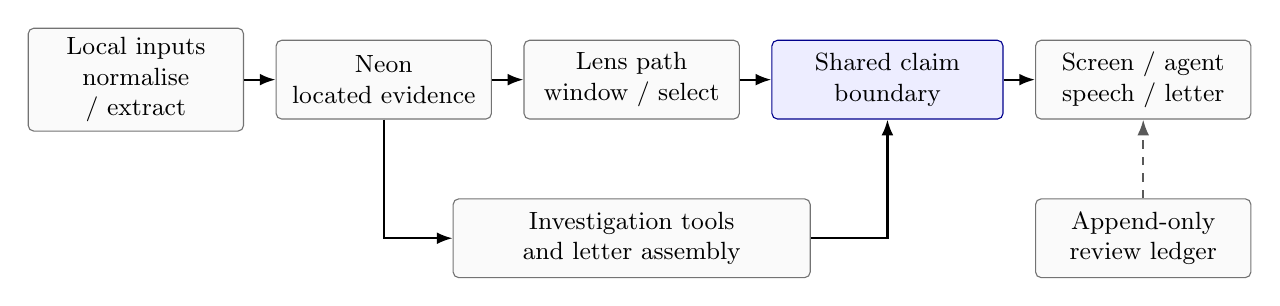
\begin{tikzpicture}[
  node distance=5mm and 4mm,
  box/.style={draw=black!55,rounded corners=2pt,align=center,font=\small,
              minimum height=10mm,text width=25mm,fill=black!2},
  gate/.style={box,fill=blue!7,draw=blue!55!black,text width=27mm},
  arrow/.style={-{Latex[length=2mm]},thick},
  overlay/.style={arrow,dashed,draw=black!65}
]
\node[box] (ingest) {Local inputs\\normalise / extract};
\node[box,right=of ingest] (db) {Neon\\located evidence};
\node[box,right=of db] (lens) {Lens path\\window / select};
\node[gate,right=of lens] (claims) {Shared claim\\boundary};
\node[box,right=of claims] (outputs) {Screen / agent\\speech / letter};
\node[box,below=10mm of lens,text width=43mm] (producers) {Investigation tools\\and letter assembly};
\node[box,below=10mm of outputs] (reviews) {Append-only\\review ledger};
\draw[arrow] (ingest) -- (db);
\draw[arrow] (db) -- (lens);
\draw[arrow] (lens) -- (claims);
\draw[arrow] (db.south) |- (producers.west);
\draw[arrow] (producers.east) -| (claims.south);
\draw[arrow] (claims) -- (outputs);
\draw[overlay] (reviews.north) -- (outputs.south);
\end{tikzpicture}
\caption{Evidence and output paths. Investigation answers and letter sentences enter the
same claim boundary as lens cards. Dashed arrows indicate review overlays on presentation;
the ledger does not rewrite evidence or machine validation results.}
\label{fig:architecture}
\end{figure}

Configured situation chips skip model parsing. Typed input is parsed into a role, task,
concerns and evidence date. A fixed needs catalog constrains planning; an unfamiliar role
can combine catalog entries but cannot invent new card semantics. Section selection calls
run in parallel under bounded request concurrency. The stream first supplies section
titles, then completed sections, checked headlines, findings and timings. Title arrival is
not counted as arrival of an answering card.

The investigation dock retrieves facts and passages, checks documentation, lists findings,
constructs timelines and computes explicitly supported arithmetic. Generated answer text
is buffered until its sentence claims pass validation. Speech uses validated text; the
server checks a signed receipt before forwarding it to the speech service. Letters use
template-first assembly and sentence validation. Editing a factual sentence retains its
citations and triggers revalidation. Unsupported clinician additions remain labelled notes.

\section{Trust model}
The following principles are requirements that evaluation must test, not guarantees that
a language model is correct.
\begin{enumerate}[label=\textbf{\arabic*.},itemsep=2pt]
\item \textbf{Located evidence.} Every stored fact has a quote located in its normalised
segment. Sensitive values, including doses, dates and laterality, must be supported by the
located text. A location failure is dropped and logged.
\item \textbf{A shared claim boundary.} Every patient-facing statement is represented as
a Claim. Template, composed and absence claims have different proof obligations. Fixed
nonclinical boilerplate is explicitly exempt; annotations never become source facts.
\item \textbf{Selection before rendering.} The screen model returns eligible fact IDs,
completeness and an optional headline. Templates render fact lines; failed headlines fall
back to those checked lines.
\item \textbf{Qualified absence.} ``Not documented'' requires both synonym search and a
full-text model check across every eligible document. A failed or timed-out check yields
``Couldn't check''. Missing documentation does not imply absence of disease.
\item \textbf{A shared evidence window.} Every component receives the same eligible set
and corpus revision. A finding appears only if all its supporting passages are eligible.
\item \textbf{Independent state dimensions.} Availability, assertion, temporal status,
completeness, conflict and review are stored separately. A documented negative result is
not a documentation gap; a planned procedure is not a completed procedure.
\item \textbf{Review as an overlay.} Accept, correct, dismiss and leave-open decisions
append ledger entries. They do not change documents, extracted facts or machine verdicts.
Evaluation uses an empty review layer.
\item \textbf{Complete cache identity.} Reuse binds patient, corpus revision, the complete
evidence window, validator version, normalised claim text, cited fact IDs with content
hashes, and segment IDs. A revision change invalidates prior evidence assumptions.
\item \textbf{Adjudicated inconsistencies.} Candidate differences require event identity
and context. Only contradictions and clarification requests appear; medication changes
between source lists are trends.
\item \textbf{Source-labelled medication.} A medication list retains its source date and
document context. It is not described as the patient's current medication.
\end{enumerate}

Location, semantic support and coverage are distinct. Exact offsets establish where text
occurs; they do not establish that an English claim preserves its meaning. Semantic checks
compare a claim with facts, original passages and neighbouring context. Coverage evaluation
asks whether the necessary answer was selected at all. A system can pass location checks
and still omit a clinically important fact or mishandle temporal meaning.

\section{Ingestion and multimodal extension}
Text normalisation decodes entities and line breaks while retaining a map to raw offsets.
The segmenter recognises headings, list items, sentences and medication rows, protecting
common German abbreviations and wrapped text. Deterministic medication parsing preserves
ordered schedule columns, units, route and weekly instructions. Structured model extraction
adds atomic facts with assertion, temporal status and event-date precision. Recall hints
improve coverage but do not replace source evidence.

Quote location precedes semantic checking. Near matches are accepted only under the
locator's similarity and sensitive-value constraints; the stored quote is the actual
located span. Semantic repair must pass location again. German negation triggers provide
an independent review signal. Terminology normalisation, entity grouping and English
segment translation retain links to the original German text. A prior ingest report
records \SegmentCount{} translated segments and \FactCount{} supported facts; concept-hint
coverage was \CoverageMatched/\CoverageTotal{} (\CoveragePercent\%). These summary counts
come from an earlier ingestion run, not a fresh ingestion performed for this report.
Concept-hint coverage is not an independently adjudicated clinical recall estimate.

The page-based extension rasterises PDFs, retains embedded text with coordinates and uses
OCR for image-only pages. It converts transcribed lines to the same normalised document
and segment representation. Page and bounding-box metadata provide a second provenance
link from a text span to the rendered page. Extraction and validation then reuse the text
pipeline. An embedding of an image can retrieve a page, but it cannot by itself establish
a located textual claim. OCR errors remain evidence-quality errors; a plausible
transcription is not verified against the physical page merely because offsets match it.
Multimodal end-to-end accuracy remains unmeasured in the results below.

\section{Hybrid retrieval and the evidence window}
For the short challenge record, the core selector receives all eligible facts of relevant
kinds. This avoids a retrieval cutoff as a source of silent omission. The hybrid extension
is intended for larger records and investigation search. It combines BM25 lexical matching
over German and English segments with vector similarity from Gemini Embedding 2.
The lexical branch uses the database search extension when available and a scoped
in-process BM25 implementation otherwise. Vector storage uses pgvector; missing embedding
credentials or vector failure can degrade retrieval to the lexical branch, with explicit
logging. No result below establishes a hybrid retrieval improvement.

The store defines knowledge-time eligibility once:
\begin{equation}
 E(p,r,t)=\{d:\operatorname{patient}(d)=p,\ \operatorname{revision}(d)=r,
                       \ \operatorname{docDate}(d)\leq t\}.
\end{equation}
Search consumes this set rather than computing another local date filter. The event date
may be later than $t$ when an eligible document describes a plan; the temporal label must
retain that distinction. Revision guards reject stale reads when ingestion replaces
stable document identifiers. Both retrieval branches restrict patient, revision and
eligible document IDs before ranking.

For rank lists $\mathcal R$, fusion assigns segment $s$ the score
\begin{equation}
 \operatorname{RRF}(s)=\sum_{R\in\mathcal R:s\in R}
                      \frac{1}{\kappa+\operatorname{rank}_R(s)},
\end{equation}
where $\kappa$ dampens individual rank positions \citep{rrf}. Duplicate segments contribute
once per branch and deterministic tie-breaking preserves reproducibility. Fused hits
remain candidates, not facts. Crucially, an empty top-ranked list never authorises an
absence claim: full-window synonym and full-text checks remain mandatory.

\section{Contradiction adjudication}
A qualifying contradiction concerns the same event or measurement and contains statements
that cannot all be true. The source must establish event identity; resemblance alone is
insufficient. Rules propose candidates from laterality, dates and arithmetic, while a model
sweep can propose contextual candidates. Explicitly proven rule cases use deterministic
classification; ambiguous and model-proposed cases require adjudication. Its taxonomy
separates contradiction, needs clarification, change over time, measurement variation,
omission and different context. Public finding
wording passes the claim boundary, including at read time, so a downgraded clarification
cannot retain an unchecked stronger explanation.

The challenge fixtures provide deliberately narrow tests. C1 concerns laterality: a
vascular findings section and its assessment attribute the same clinically relevant
stenosis to different sides. C2 and C3 compare recorded BMI with the height and weight
recorded alongside it; rounding intervals determine whether the values can be consistent.
C4 compares collection dates for a biopsy linked across a letter and pathology report.
C5 concerns incompatible dates for the same discharge, including an apparent year typo.
These are English paraphrases; source text is not reproduced.

D1 preserves different admission dates because hospital and ward admission may be distinct.
D2 retains an unresolved difference in axillary-node findings because examinations,
dates and anatomical context are not established as identical. D3 concerns case identifiers
whose common scope has not been demonstrated. These are clarification requests, not
additional contradictions. Weight changes, small height or blood-pressure differences,
medication schedule changes and omitted reaction details are dismissal controls. Possible
explanations remain hypotheses on the finding and do not enter the factual timeline.

\section{Synthetic data generator}
The research protocol separates a structured history from its documentation. First,
stable events and dates define a synthetic patient journey. A documentation plan specifies
what each note states, repeats, omits or negates. Templates render structured sections;
prose may be rewritten separately. Controlled mutations then introduce changes in side,
dose, date, assertion, schedule or arithmetic consistency. A mutation ledger identifies
the affected document, span and before/after value. Final labels must describe the final
normalised documents, not the latent patient history.

The shared format stores patient records in JSONL shards, with a patient index and a
manifest recording seeds, generation families, splits and held-out inventories. A
materialisation adapter produces the same directory structure as the core corpus loader.
This allows synthetic records to exercise ordinary ingestion rather than a separate
evaluation-only input route. The scale target is \SynthTarget{} patients; the current
full-corpus artifact count is \SynthPatients{}; the separate sample contains
\SynthSamplePatients{} patients. A generated count does not establish independent
label quality or linguistic diversity.

Labels have four provenance tiers: \emph{intended} from plans and mutations;
\emph{candidate} from an independent extractor; \emph{verified} after checking final spans
and independently confirming the statement; and \emph{gold} after human review.
Exact span agreement alone does not promote an intended label to verified semantic truth.
If a planned fact is omitted from every final note, its documentation label is absent.
The model being evaluated must not generate its own reference answers.

Splits are assigned by patient and generation family before augmentation. Whole writing
styles, scenario families and mutation types should be held out, with the actual inventory
recorded in the manifest. Paraphrases and mutated siblings remain in the same partition.
Near-duplicate checks and a human sample are needed because family-level splits do not
guarantee linguistic independence. In particular, a large template corpus can have a much
smaller effective diversity than its patient count suggests.

\section{Own verifier: dataset, adaptation and baselines}
The specialised task is evidence-conditioned claim classification: supported,
unsupported or contradicted, with assertion and timing as additional labels. Inputs pair
an English claim with German source segments, headings and immediate context. Supported
examples are rendered from final-document facts; controlled perturbations create
incompatible claims, and absent additions supply unsupported cases. Mutation provenance
must remain distinguishable from human adjudication.

The experimental dataset builder checks final quote offsets, groups patients and families
before augmentation, respects declared held-out partitions and records split assignments.
Its labels are intended plus final-span-checked, not human gold. Balanced sampling aids
comparison across classes but changes deployment prevalence; accuracy on this distribution
cannot estimate clinical error rates directly. The recorded training, validation and test
sizes are \TrainExamples{}, \ValidationExamples{} and \TestExamples{}, respectively.

The local MLX experiment trains low-rank adapters on a frozen quantized base model.
This follows the quantized-adaptation idea of QLoRA, without claiming reproduction of all
the numerical and optimizer details in \citet{qlora}. Training records the base model,
adapter configuration, token limit, seed, completed iterations and wall-clock status.
Examples exceeding the configured context limit are rejected rather than truncating away
their label evidence. A training command or allocated model is not evidence of a completed
training run.

Inference compares candidate label-completion likelihoods. Their normalised scores are
closed-set, uncalibrated values, not probabilities that a clinical statement is true.
Evaluation should compare rules-only checks, the proxy semantic verifier, the unadapted
local model and its adapted counterpart on identical held-out examples. Report classwise
precision/recall, macro F-score, confusion matrices, abstention coverage and latency.
Assertion and timing sub-labels require separate scores. Integration into the shared claim
boundary is a distinct experiment; a local endpoint does not establish that every
production claim uses it.

\section{Evaluation}
\subsection{Challenge record and observed machine results}
The so-called real-patient regression is a realistic challenge workflow over a synthetic
patient, not a study involving a real clinical cohort. It contains \RegressionTarget{}
questions across \SituationCount{} configured situations. An answer counts only when the
relevant card is rendered and cites an expected source, except for fully checked
documentation gaps. The engine/API judge and browser visibility checks answer different
questions and must be reported separately. Every run uses an empty review overlay and
rejects labelled mock fallback.

Table~\ref{tab:results} aggregates a complete saved live result bundle. Newer standalone
regression scores are not combined with its audits or timings. Answer-and-citation passes differ
from whole-suite passes because availability and invariant checks also contribute to the
suite. Located fact references are repeated uses, not distinct facts. The composed-claim
audit checked \ComposedChecked{} claims, so it does not establish composed-claim precision
when that count is empty. Fixture recovery concerns the specified challenge controls, not
open-world inconsistency recall or specificity. Human verification is still required
before treating these values as submission metrics.

\begin{table}[htbp]
\centering\small
\begin{tabular}{@{}p{.62\linewidth}r@{}}
\toprule
Measure & Observed \\
\midrule
Primary cold answers (text and chip, each) & \ReviewedAnswerPassed/\ReviewedAnswerTotal \\
Cited facts located / checked & \ReviewedTraceLocated/\ReviewedTraceTotal \\
Unsupported / distinct card lines reviewed & \ReviewedUnsupported/\ReviewedLines \\
True contradictions / false findings & \ReviewedContradictions/\ReviewedFalseAlarms \\
Slowest primary cold API completion (s) & \ReviewedColdSeconds \\
Slowest confirmed cached API completion (s) & \ReviewedCachedSeconds \\
\bottomrule
\end{tabular}

\caption{Saved automated observations from a live regression run. Pending denotes an
absent or inapplicable measurement, including browser visibility and confirmed cache
latency. These values are not human-checked clinical results.}
\label{tab:results}
\end{table}

\subsection{Held-out tasks and synthetic challenges}
The held-out protocol contains \HeldoutTarget{} situations, reported by generalisation
tier: reworded configured tasks, new combinations of known needs, and roles without a
profile. Scores remain unopened until the project's checkpoint permits review. The
default number-generation command does not read the protected held-out file.
Table~\ref{tab:heldout} therefore keeps unavailable tier results pending rather than
substituting regression performance.

\begin{table}[htbp]
\centering\small
\begin{tabular}{@{}p{.62\linewidth}r@{}}
\toprule
Generalisation tier & Relevance / grounding passes \\
\midrule
Reworded configured situation & \TierOneRelevance{} / \TierOneGrounding{} (\TierOneCount{}) \\
New combination of known needs & \TierTwoRelevance{} / \TierTwoGrounding{} (\TierTwoCount{}) \\
Role without a configured profile & \TierThreeRelevance{} / \TierThreeGrounding{} (\TierThreeCount{}) \\
\bottomrule
\end{tabular}

\caption{Held-out relevance and grounding passes, with tier sample counts in parentheses.
Pending cells preserve the checkpoint restriction or indicate missing results.}
\label{tab:heldout}
\end{table}

The scale evaluation protocol requires at least \ChallengeMinimum{} synthetic challenges,
covering laterality, dose and date changes, negation, temporal status, arithmetic,
documentation gaps and benign distractors. Generation-family and mutation holdouts must
be preserved. A challenge only counts as evaluated when its execution and scoring finish;
an enumerated challenge file is not a performance result. Retrieval should be evaluated
against labelled supporting spans using recall at a declared cutoff and reciprocal rank,
with BM25-only, vector-only, fused and exhaustive-selection baselines. End-to-end answer
quality and absence correctness remain separate from retrieval recall.

\begin{table}[htbp]
\centering\small
\begin{tabular}{@{}p{.62\linewidth}r@{}}
\toprule
Research artifact & Observed \\
\midrule
Generated synthetic patients & \SynthPatients \\
Generated synthetic documents & \SynthDocuments \\
Code-checked facts / contradictions & \SynthFacts / \SynthContradictions \\
Distractors / documentation gaps & \SynthDistractors / \SynthGaps \\
Patients with rewritten prose & \SynthRewrittenPatients \\
Sample patients / documents & \SynthSamplePatients / \SynthSampleDocuments \\
Synthetic challenges generated & \SyntheticGenerated \\
Synthetic challenges evaluated & \SyntheticChallenges \\
Verifier training / validation / test examples & \TrainExamples / \ValidationExamples / \TestExamples \\
Verifier macro F-score & \VerifierMacroFone \\
Verifier accuracy & \VerifierAccuracy \\
Verifier median latency (ms) & \VerifierLatencyMs \\
Retrieval recall at configured cutoff & \RetrievalRecall \\
\bottomrule
\end{tabular}

\caption{Research artifact aggregates. Pending inputs remain pending; no scale, retrieval
or verifier performance is imputed from an implementation or target.}
\label{tab:research}
\end{table}

\begin{table}[htbp]
\centering\small
\begin{tabular}{@{}lrrrr@{}}
\toprule
Verifier & Examples & Macro F-score & Coverage & Median ms \\
\midrule
Rules only & \RulesVerifierN & \RulesVerifierFscore & \RulesVerifierCoverage & \RulesVerifierLatency \\
Proxy semantic & \ProxyVerifierN & \ProxyVerifierFscore & \ProxyVerifierCoverage & \ProxyVerifierLatency \\
Local adapter & \LocalVerifierN & \LocalVerifierFscore & \LocalVerifierCoverage & \LocalVerifierLatency \\
Local + GPT cascade & \CascadeVerifierN & \CascadeVerifierFscore & \CascadeVerifierCoverage & \CascadeVerifierLatency \\
\bottomrule
\end{tabular}

\caption{Verifier baselines on held-out synthetic generation families. Scores are fractions;
coverage counts valid model outputs. Missing methods and empty evaluation sets remain pending.}
\label{tab:verifier}
\end{table}

\begin{table}[htbp]
\centering\small
\begin{tabular}{@{}lrrrr@{}}
\toprule
Retrieval & Queries & Recall@$5$ & Recall@$10$ & MRR@$10$ \\
\midrule
BM25 & \LexicalRetrievalN & \LexicalRecallFive & \LexicalRecallTen & \LexicalMrrTen \\
Vector & \VectorRetrievalN & \VectorRecallFive & \VectorRecallTen & \VectorMrrTen \\
Hybrid & \HybridRetrievalN & \HybridRecallFive & \HybridRecallTen & \HybridMrrTen \\
\bottomrule
\end{tabular}

\caption{Retrieval baselines on labelled spans. A hybrid result can be a lexical fallback;
the run metadata must establish embedding availability before a hybrid benefit is claimed.}
\label{tab:retrieval}
\end{table}

\subsection{Latency and reproducibility}
Measure submission-to-first-answering-card and submission-to-final-section separately,
alongside model, database and validation time. The protocol targets \FirstCardTarget{}
seconds for the first card, \ColdTarget{} seconds for a complete cold screen and
\CachedTarget{} second for confirmed cache replay; the challenge ceiling is
\ChallengeLimit{} seconds. These limits are targets; missing timing cells do not
establish compliance. Warm requests without cache confirmation do not measure
cache replay. Browser timing remains pending when the browser cannot complete its checks.

The paper build records input paths and content hashes in generated provenance metadata.
It exports aggregate numeric fields only, never patient passages, judge explanations or
predictions. A malformed, absent or mock-only input cannot become a reported clinical
result. Regeneration checks that audit metadata matches the scored rows, preventing
accidental combination of different runs. This binds the PDF to a saved evidence snapshot;
it does not make that snapshot representative of later concurrent code changes.

\FloatBarrier
\section{Limitations}
The challenge corpus is small, synthetic and actively used for development. Its regression
score is not an estimate of clinical generalisation. Templates constrain output but can
still propagate extraction errors or omit qualifications. Model-based support and absence
checks can share systematic errors with extraction and evaluation, especially when model
roles share a family. A complete-document prompt does not prove semantic exhaustiveness.

The live results expose incomplete end-to-end correctness and latency above target.
Browser visibility, multimodal accuracy, synthetic challenge performance and trained
verifier benefits need completed measurements. Research extensions are developed
concurrently; code presence is weaker evidence than a reproducible run. Label balance,
simple perturbations and repetitive templates can inflate verifier scores. Family holdouts
and independent human labels are necessary but do not establish transfer to authentic
records, institutions, dialects or rare events.

The single evidence window uses document time, not a complete bitemporal clinical model.
Late-entered notes, amended records and uncertain dates require richer modelling.
Source-linked English text can also change nuance in translation. Reviews improve
inspectability but do not make an unsupported clinician statement source-supported.
The prototype has not established clinical effectiveness or safety for care decisions.

\section{Ethics and data handling}
Challenge documents are loaded locally at runtime and never published with this paper,
its source, fixtures or generated tables. The repository blocks challenge directories,
archives, dumps and secrets, and scans staged content for copied passages. Fixture
descriptions above are English paraphrases without German document quotations. Synthetic
training data must be generated independently rather than obtained by rewriting challenge
notes. Public release decisions must distinguish newly generated examples from protected
challenge material.

The prototype uses external model, storage and optional speech services; local verifier
inference does not make the complete system on-premises. Research use of authentic records
would require an appropriate legal basis, access governance, retention policy and
institutional review. Human authorship and clinical acceptance remain separate from
document support. Missing evidence and unresolved conflicts are surfaced for review;
neither is silently converted into reassurance.

\bibliographystyle{plainnat}
\bibliography{refs}
\end{document}
